\section{Casos de uso}

\subsection{Diagramas de casos de uso}
\begin{figure}[H]
    \centering
    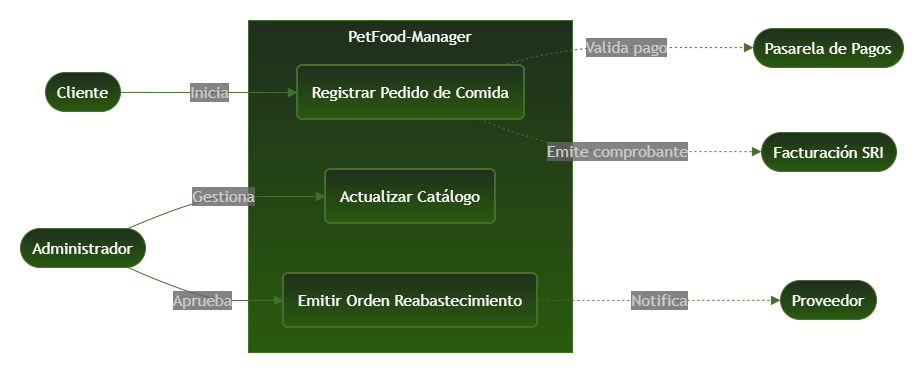
\includegraphics[width=0.60\textwidth]{Images/diagramaCasosUsos.png}
    \caption{Diagrama de Casos de Uso General}
    \label{fig:cu_general}
\end{figure}

\begin{figure}[H]
    \centering
    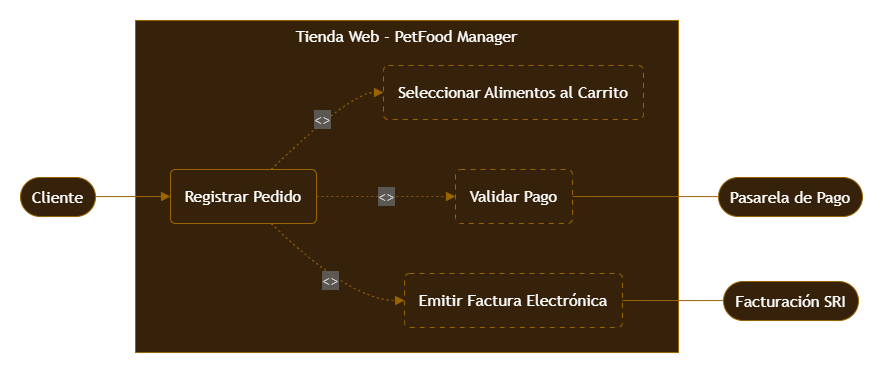
\includegraphics[width=0.60\textwidth]{Images/registroPedidoClase.png}
    \caption{Diagrama de Caso de Uso Específico 1}
    \label{fig:cu_especifico_1}
\end{figure}

\begin{figure}[H]
    \centering
    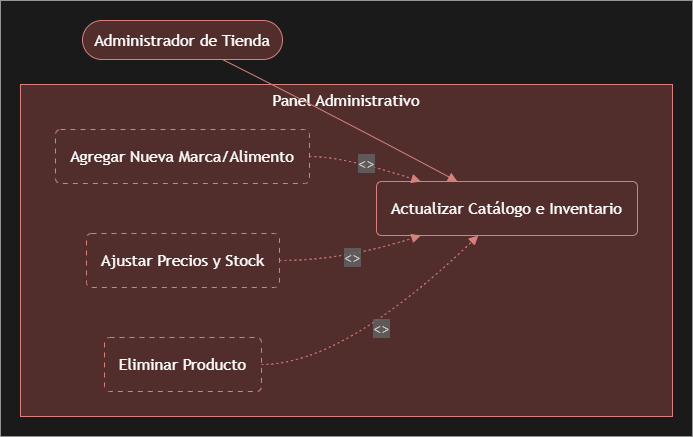
\includegraphics[width=0.60\textwidth]{Images/actualizarCatalogoClase.png}
    \caption{Diagrama de Caso de Uso Específico 2}
    \label{fig:cu_especifico_2}
\end{figure}

\begin{figure}[H]
    \centering
    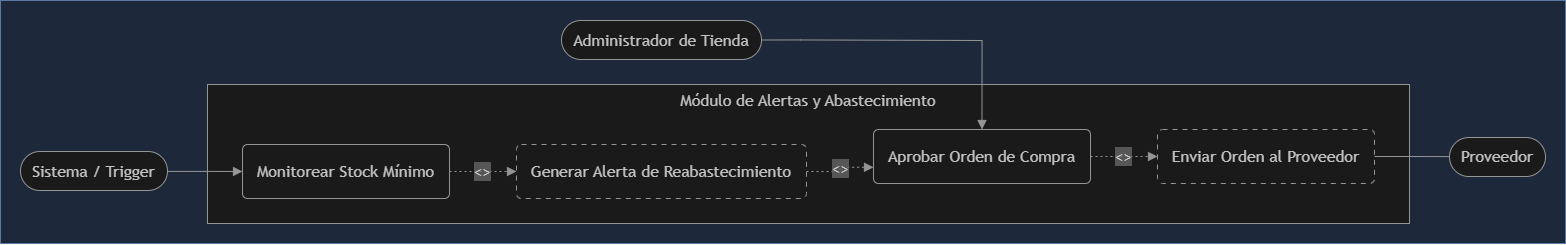
\includegraphics[width=0.60\textwidth]{Images/alertaRebstecimientoClase.png}
    \caption{Diagrama de Caso de Uso Específico 3}
    \label{fig:cu_especifico_3}
\end{figure}

\newpage
\subsection{Especificación de casos de uso}

\begin{table}[H]
    \centering
    \small
    \renewcommand{\arraystretch}{1.4}
    \begin{tabularx}{\textwidth}{|>{\bfseries\raggedright\arraybackslash}p{4cm}|L|}
        \hline
        \rowcolor{upsblue} \multicolumn{2}{|c|}{\textcolor{white}{\textbf{Especificación de Caso de Uso 1}}} \\
        \hline
        Nombre del caso de uso & Registrar Pedido de Comida de Mascotas \\
        \hline
        Descripción & El cliente selecciona comida para su mascota de la tienda web e ingresa datos de pago y envío para generar el pedido. \\
        \hline
        Precondición & El cliente debe estar logueado y el catálogo debe tener existencias (stock) del alimento deseado. \\
        \hline
        Actores & Cliente (iniciador), Pasarela de Pago, Administrador de Tienda (receptor). \\
        \hline
        Secuencia normal & 
        1. El cliente examina y selecciona la marca de comida y el tamaño de bolsa (kg). \par
        2. El cliente añade los productos al carrito de compras y pulsa ``Proceder al Pago''. \par
        3. El sistema solicita los datos de envío y dirige a la Pasarela de Pago. \par
        4. El cliente ingresa su método de pago y autoriza la transacción. \par
        5. El sistema valida la transacción, descuenta el stock y genera la orden de despacho. \\
        \hline
        Poscondición & El stock se reduce en la base de datos, se envía correo de confirmación de pedido y comprobante electrónico al cliente. \\
        \hline
        Excepciones & 
        4.a. Transacción rechazada por fondos insuficientes: El sistema indica el error y retorna al carrito de compras. \par
        5.a. Fallo en la comunicación con el SRI para facturación: El sistema almacena la factura como offline y la reintenta luego. \\
        \hline
        Importancia & Alta \\
        \hline
    \end{tabularx}
    \caption{Especificación de Caso de Uso 1: Registrar Pedido}
    \label{tab:especificacion_cu1}
\end{table}

\newpage
\begin{table}[H]
    \centering
    \small
    \renewcommand{\arraystretch}{1.4}
    \begin{tabularx}{\textwidth}{|>{\bfseries\raggedright\arraybackslash}p{4cm}|L|}
        \hline
        \rowcolor{upsblue} \multicolumn{2}{|c|}{\textcolor{white}{\textbf{Especificación de Caso de Uso 2}}} \\
        \hline
        Nombre del caso de uso & Actualizar Catálogo e Inventario de Alimentos \\
        \hline
        Descripción & El administrador del negocio registra nuevas marcas, bolsas de comida o ajusta stock y precios del catálogo de la tienda. \\
        \hline
        Precondición & El usuario administrador debe haberse autenticado correctamente en el panel administrativo. \\
        \hline
        Actores & Administrador de Tienda. \\
        \hline
        Secuencia normal & 
        1. El administrador ingresa a ``Gestión de Inventario'' y presiona ``Agregar Producto''. \par
        2. Completa el formulario con: nombre del alimento, marca, animal destinatario, peso, precio de venta, stock actual y stock mínimo. \par
        3. El administrador sube la imagen del producto y pulsa ``Guardar''. \par
        4. El sistema valida los datos y registra el producto en la base de datos. \\
        \hline
        Poscondición & El catálogo público de la tienda se actualiza con el nuevo alimento y cantidad disponible. \\
        \hline
        Excepciones & 
        2.a. El stock ingresado es un número negativo: El sistema bloquea el guardado y muestra mensaje de error. \par
        3.a. Imagen supera el formato o peso máximo: El sistema pide subir una imagen optimizada. \\
        \hline
        Importancia & Alta \\
        \hline
    \end{tabularx}
    \caption{Especificación de Caso de Uso 2: Actualizar Catálogo}
    \label{tab:especificacion_cu2}
\end{table}

\newpage
\begin{table}[H]
    \centering
    \small
    \renewcommand{\arraystretch}{1.4}
    \begin{tabularx}{\textwidth}{|>{\bfseries\raggedright\arraybackslash}p{4cm}|L|}
        \hline
        \rowcolor{upsblue} \multicolumn{2}{|c|}{\textcolor{white}{\textbf{Especificación de Caso de Uso 3}}} \\
        \hline
        Nombre del caso de uso & Emitir Orden de Reabastecimiento Automática \\
        \hline
        Descripción & El sistema genera una alerta visual y un reporte de orden de compra para un proveedor cuando el inventario baja de su stock mínimo. \\
        \hline
        Precondición & El stock del artículo es inferior al stock crítico establecido en el inventario. \\
        \hline
        Actores & Sistema (iniciador), Administrador de Tienda (aprobador), Proveedor de Alimentos (receptor). \\
        \hline
        Secuencia normal & 
        1. Tras confirmarse una venta, el sistema detecta que el stock disponible es menor que el stock mínimo configurado. \par
        2. El sistema genera automáticamente un borrador de Orden de Compra dirigida al proveedor asociado. \par
        3. El sistema muestra una alerta en el dashboard del Administrador. \par
        4. El administrador abre la alerta, revisa los kilos sugeridos de alimento a pedir y pulsa ``Aprobar Orden''. \par
        5. El sistema despacha el correo electrónico formal con la orden de compra al sistema del Proveedor. \\
        \hline
        Poscondición & El sistema registra el estado del lote en ``Pendiente de Arribo'' y el proveedor recibe el requerimiento. \\
        \hline
        Excepciones & 
        2.a. No hay un proveedor asociado a esa marca de comida de mascotas: El sistema genera una alerta solicitando la asignación manual de un proveedor. \par
        4.a. El administrador edita la cantidad antes de enviar: El sistema recalcula los valores de la orden. \\
        \hline
        Importancia & Media \\
        \hline
    \end{tabularx}
    \caption{Especificación de Caso de Uso 3: Alerta de Reabastecimiento}
    \label{tab:especificacion_cu3}
\end{table}